\section{Results and Discussion}

In order to broadly assess the selective consequences of each treatment with respect to the functional and reproductive cooperation characteristic of evolutionary transitions of individuality, we begin with aggregate analysis of the relationship between same-channel signaling network context and resource-sharing and cell reproduction behavior.
Then, in section \ref{sec:life-histories} we will survey observed multicellular life histories.

Subsequent sections describe the mechanistic underpinnings and fitness effects of notable phenotypic traits that evolved in individual replicates.
Section \ref{sec:gene-regulation} reports an endogenous propagule-seeding strategy mediated by gene regulation.
Section \ref{sec:gradient-conditioned-behavior} describes cell behavior plastically conditioned by a resource gradient.
Section \ref{sec:morphology} details a stringy same-channel signaling network morphology.
Section \ref{sec:cell-cell-messaging} provides two examples of adaptive cell-cell messaging.
Finally, section \ref{sec:apoptosis} reviews two replicates where widespread apoptosis evolved.

\subsection{Reproductive Cooperation} \label{sec:reproductive-cooperation}

\begin{figure}[!htbp]
\begin{center}

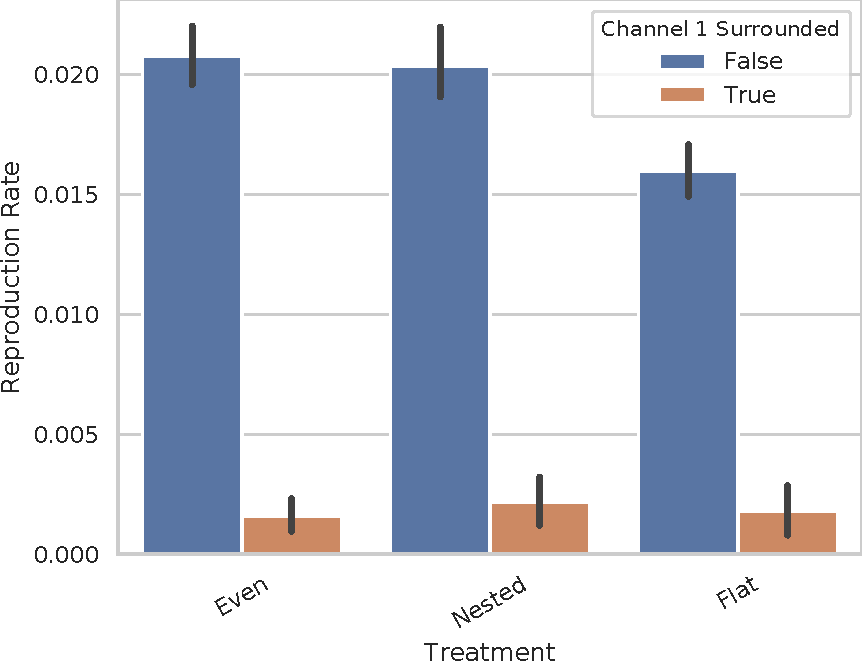
\includegraphics[width=\columnwidth]{reproduction/title=reproductive_labor_surrounded+_data_hathash_hash=4e1be4c5abfa4b05+_script_fullcat_hash=62ec0af515e8429d+_source_hash=ffbe01c-clean+ext=}

\caption{
TODO
}
\label{fig:reproduction_surrounted}
\end{center}
\end{figure}


Figure \ref{fig:reproduction_surrounded} shows cellular reproduction rates based on context in highest-level same-channel signaling networks.
In the nested and even treatments, this corresponded to the level-one channel and, in the flat treatment where no level-one channel was defined, this corresponded to the level-zero channel.
For all treatments, phenotypes with depressed interior cellular reproduction rates dominated across replicates ($p < 0.05$; $n=40$; bootstrap test).
[TODO just lookin' at non-overlapping 95\% CI's y'all]
All three treatments appear to be sufficient to select for reproductive cooperation among cells.

\subsection{Resource Sharing} \label{sec:resource-sharing}

\begin{figure*}[!htbp]
\begin{center}

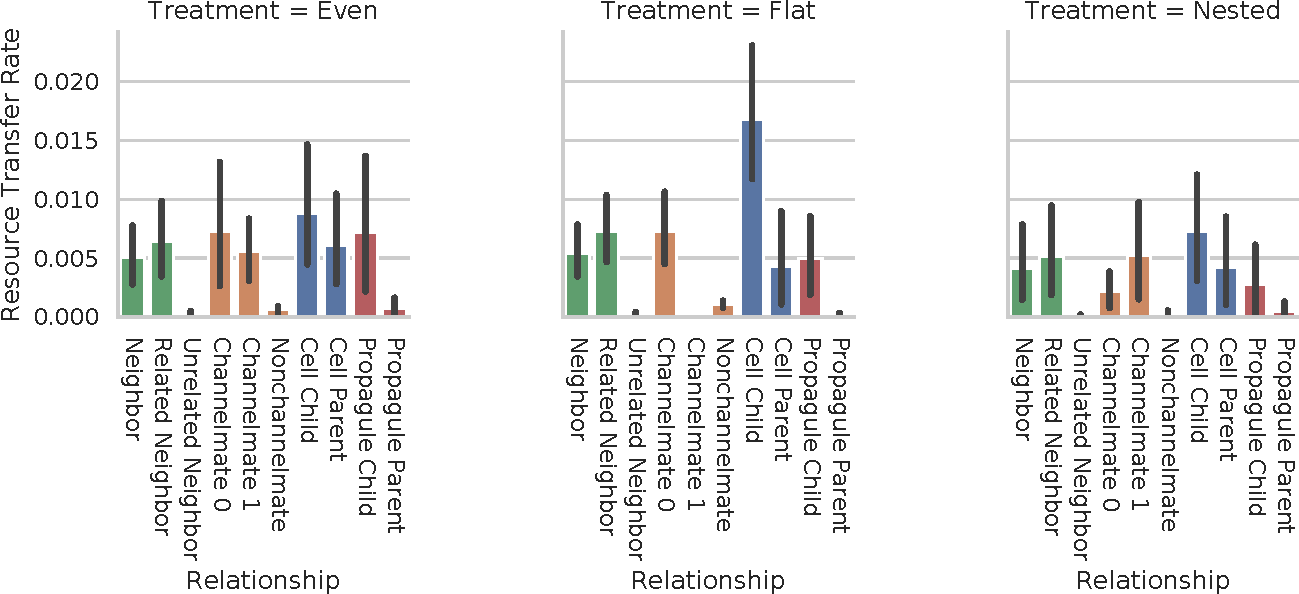
\includegraphics[width=\textwidth]{sharing/title=Resource_Transfer_Rate+_data_hathash_hash=e07865a0aee42cf7+_script_fullcat_hash=3612aad527ec4368+_source_hash=ffbe01c-clean+ext=}

\caption{
TODO
}
\label{fig:sharing}
\end{center}
\end{figure*}

\begin{figure*}[!htbp]
\begin{center}

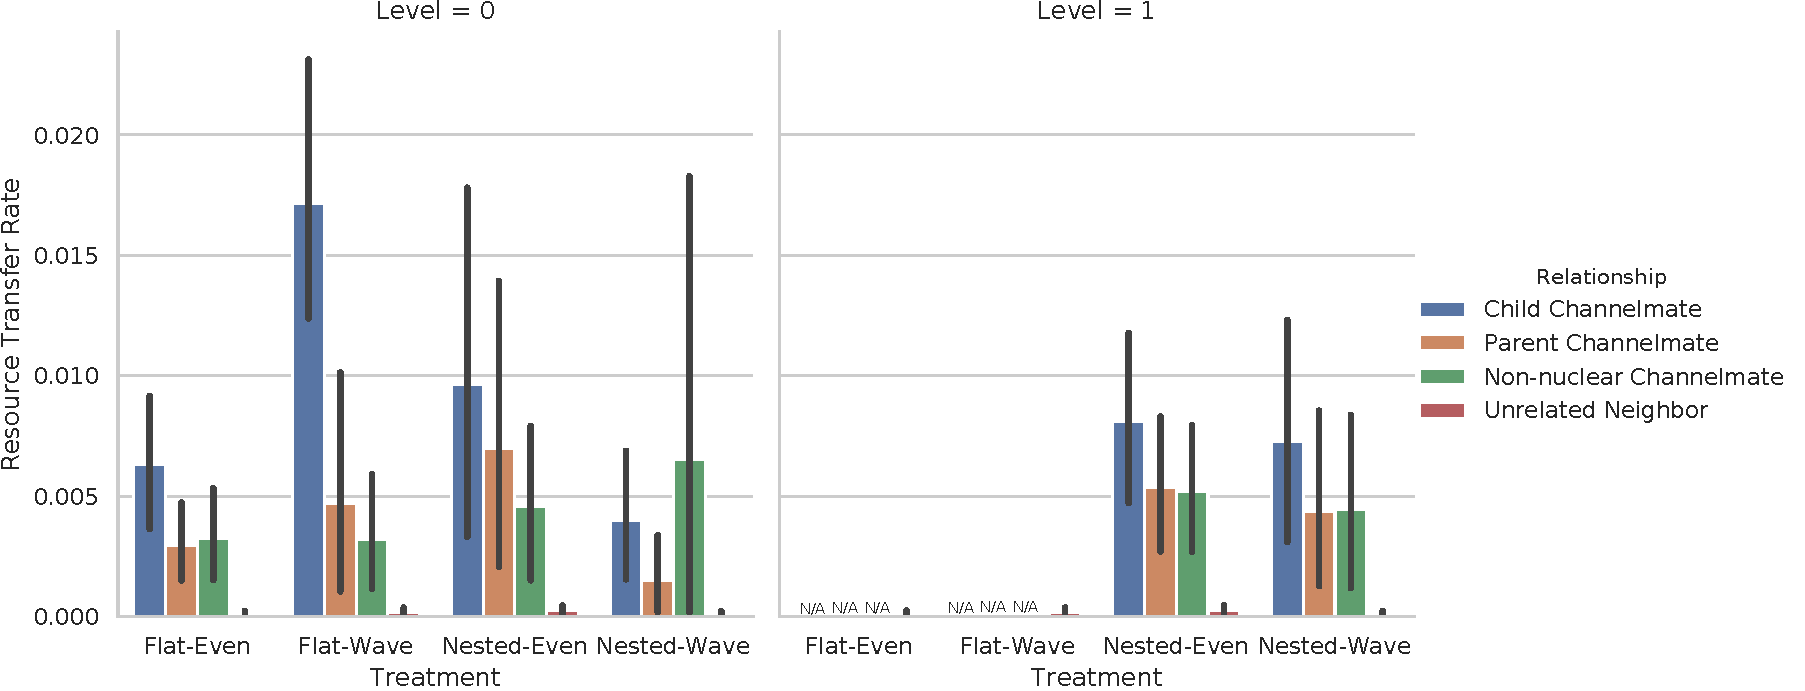
\includegraphics[width=\textwidth]{sharing/title=Resource_Transfer_Rate+_data_hathash_hash=2137e250b9d2b681+_script_fullcat_hash=86edbf4a4e5f34ed+_source_hash=53a2252-clean+ext=}

\caption{
Resource sharing to mutually exclusive sub-categories same-channel cellular neighbors: cellular child, cellular parent, and neither (``non-nuclear'').
Resource sharing to entirely non-related cells (no cell, channel, or propagule relation) is included for comparison.
Note that level-one groups are not defined in either of the flat treatments.
Error bars indicate 95\% confidence.
}
\label{fig:sharing_channelmate}
\end{center}
\end{figure*}


Figure \ref{fig:sharing} overviews evolved resource sharing behavior across cellular contexts.

Replicates in the flat treatment exhibit an especially elevated rate of resource sharing to cell children.
This could perhaps be due to an especial selective pressure to convey resource towards the group periphery.

Also, in the even and flat treatments, more resource was shared to neighbors within a cell's same-channel signaling network's propagule than to an unrelated neighbor ($p < 0.05$; $n=40$; bootstrap test).
Functional cooperation to directly further group reproduction therefore appears to have evolved commonly under these treatments.

Surprisingly, in the nested treatment resource was shared at a higher mean rate among high-level same-channel signaling groups than low-level groups.
This observation is likely due to replicates where level-one same-channel signaling groups were composed of single-cell level-zero same-channel signaling groups (where no or very few opportunities for level-zero resource sharing occurred).

Finally, under all treatments resource was transferred to channelmates at a significantly higher mean rate than to unrelated neighbors ($p < 0.05$; $n=40$; bootstrap test).
[TODO just lookin' at non-overlapping 95\% CI's y'all]
This observation suggests that functional cooperation within same-channel groups might have been a common evolutionary outcome under all three treatments.
However, it could potentially be an artifact of resource sharing between direct cellular kin.

Figure \ref{fig:sharing_channelmate} breaks same-channel resource-sharing apart by cellular kin relation.
In all three treatments, mean sharing to direct-kin channelmates was indeed greater than to other channelmates.
This cold be due to an evolutionary incentive to favor direct cell kin over other channelmates, group-level selection for asymmetric resource flow achieved by preferential sharing, or some combination of the two.
However, in all three treatments mean sharing to non-direct-kin channelmates was also significantly greater than resource sharing to unrelated neighbors ($p < 0.05$; $n=40$; bootstrap test).
[TODO just lookin' at non-overlapping 95\% CI's y'all]
Thus, all three treatments appear to be sufficient to select for functional cooperation among cells.

\subsection{Case Studies: Life Histories} \label{sec:life-histories}

Although functional and reproductive cooperation was ubiquitous among same-channel signaling networks, across replicates these outcomes were realized via diverse set of qualitiative life histories.
\begin{figure*}[!htbp]
\begin{center}

\begin{subfigure}[b]{\textwidth}
\centering
\begin{minipage}[t]{0.18\textwidth}
\centering
\adjincludegraphics[width=\textwidth, trim={{.66\width} {.66\width} {.0\width} {.0\width}}, clip]{lifecycle/transfer-paint/seed=1004+title=directional_propagule_viz+treat=resource-wave__channelsense-yes__nlev-two+update=1048896+_data_hathash_hash=06a65518d5588ef3+_script_fullcat_hash=8b1f57a580a67198+_source_hash=ffbe01c-clean+ext=}
Update 0
\end{minipage}
\begin{minipage}[t]{0.18\textwidth}
\centering
\adjincludegraphics[width=\textwidth, trim={{.66\width} {.66\width} {.0\width} {.0\width}}, clip]{lifecycle/transfer-paint/seed=1004+title=directional_propagule_viz+treat=resource-wave__channelsense-yes__nlev-two+update=1048928+_data_hathash_hash=06a65518d5588ef3+_script_fullcat_hash=8b1f57a580a67198+_source_hash=ffbe01c-clean+ext=}
Update 32
\end{minipage}
\begin{minipage}[t]{0.18\textwidth}
\centering
\adjincludegraphics[width=\textwidth, trim={{.66\width} {.66\width} {.0\width} {.0\width}}, clip]{lifecycle/transfer-paint/seed=1004+title=directional_propagule_viz+treat=resource-wave__channelsense-yes__nlev-two+update=1048960+_data_hathash_hash=06a65518d5588ef3+_script_fullcat_hash=8b1f57a580a67198+_source_hash=ffbe01c-clean+ext=}
Update 64
\end{minipage}
\begin{minipage}[t]{0.18\textwidth}
\centering
\adjincludegraphics[width=\textwidth, trim={{.66\width} {.66\width} {.0\width} {.0\width}}, clip]{lifecycle/transfer-paint/seed=1004+title=directional_propagule_viz+treat=resource-wave__channelsense-yes__nlev-two+update=1049024+_data_hathash_hash=06a65518d5588ef3+_script_fullcat_hash=8b1f57a580a67198+_source_hash=ffbe01c-clean+ext=}
Update 128
\end{minipage}
\begin{minipage}[t]{0.18\textwidth}
\centering
\adjincludegraphics[width=\textwidth, trim={{.66\width} {.66\width} {.0\width} {.0\width}}, clip]{lifecycle/transfer-paint/seed=1004+title=directional_propagule_viz+treat=resource-wave__channelsense-yes__nlev-two+update=1049408+_data_hathash_hash=06a65518d5588ef3+_script_fullcat_hash=8b1f57a580a67198+_source_hash=ffbe01c-clean+ext=}
Update 512
\end{minipage}
\caption{Spawn TODO}
\label{fig:TODO}
\end{subfigure}

\vspace{3ex}

\begin{subfigure}[b]{\textwidth}
\centering
\begin{minipage}[t]{0.18\textwidth}
\centering
\adjincludegraphics[width=\textwidth, trim={{.0\width} {.0\width} {.66\width} {.66\width}}, clip]{lifecycle/replace-paint/seed=1023+title=directional_propagule_viz+treat=resource-wave__channelsense-yes__nlev-two+update=1048576+_data_hathash_hash=39aa6b64134daefa+_script_fullcat_hash=8b1f57a580a67198+_source_hash=ffbe01c-clean+ext=}
Update 0
\end{minipage}
\begin{minipage}[t]{0.18\textwidth}
\centering
\adjincludegraphics[width=\textwidth, trim={{.0\width} {.0\width} {.66\width} {.66\width}}, clip]{lifecycle/replace-paint/seed=1023+title=directional_propagule_viz+treat=resource-wave__channelsense-yes__nlev-two+update=1048648+_data_hathash_hash=39aa6b64134daefa+_script_fullcat_hash=8b1f57a580a67198+_source_hash=ffbe01c-clean+ext=}
Update 72
\end{minipage}
\begin{minipage}[t]{0.18\textwidth}
\centering
\adjincludegraphics[width=\textwidth, trim={{.0\width} {.0\width} {.66\width} {.66\width}}, clip]{lifecycle/replace-paint/seed=1023+title=directional_propagule_viz+treat=resource-wave__channelsense-yes__nlev-two+update=1048720+_data_hathash_hash=39aa6b64134daefa+_script_fullcat_hash=8b1f57a580a67198+_source_hash=ffbe01c-clean+ext=}
Update 144
\end{minipage}
\begin{minipage}[t]{0.18\textwidth}
\centering
\adjincludegraphics[width=\textwidth, trim={{.0\width} {.0\width} {.66\width} {.66\width}}, clip]{lifecycle/replace-paint/seed=1023+title=directional_propagule_viz+treat=resource-wave__channelsense-yes__nlev-two+update=1048792+_data_hathash_hash=39aa6b64134daefa+_script_fullcat_hash=8b1f57a580a67198+_source_hash=ffbe01c-clean+ext=}
Update 216
\end{minipage}
\begin{minipage}[t]{0.18\textwidth}
\centering
\adjincludegraphics[width=\textwidth, trim={{.0\width} {.0\width} {.66\width} {.66\width}}, clip]{lifecycle/replace-paint/seed=1023+title=directional_propagule_viz+treat=resource-wave__channelsense-yes__nlev-two+update=1048864+_data_hathash_hash=39aa6b64134daefa+_script_fullcat_hash=8b1f57a580a67198+_source_hash=ffbe01c-clean+ext=}
Update 288
\end{minipage}
\caption{Replace TODO}
\label{fig:TODO}
\end{subfigure}

\vspace{3ex}

\begin{subfigure}[b]{\textwidth}
\centering
\begin{minipage}[t]{0.18\textwidth}
\centering
\adjincludegraphics[width=\textwidth, trim={{.0\width} {.66\width} {.66\width} {.0\width}}, clip]{lifecycle/burst-paint/seed=1034+title=directional_propagule_viz+treat=resource-wave__channelsense-yes__nlev-two+update=1048648+_data_hathash_hash=02a94757e9b17a36+_script_fullcat_hash=8b1f57a580a67198+_source_hash=ffbe01c-clean+ext=}
Update 0
\end{minipage}
\begin{minipage}[t]{0.18\textwidth}
\centering
\adjincludegraphics[width=\textwidth, trim={{.0\width} {.66\width} {.66\width} {.0\width}}, clip]{lifecycle/burst-paint/seed=1034+title=directional_propagule_viz+treat=resource-wave__channelsense-yes__nlev-two+update=1048744+_data_hathash_hash=02a94757e9b17a36+_script_fullcat_hash=8b1f57a580a67198+_source_hash=ffbe01c-clean+ext=}
Update 96
\end{minipage}
\begin{minipage}[t]{0.18\textwidth}
\centering
\adjincludegraphics[width=\textwidth, trim={{.0\width} {.66\width} {.66\width} {.0\width}}, clip]{lifecycle/burst-paint/seed=1034+title=directional_propagule_viz+treat=resource-wave__channelsense-yes__nlev-two+update=1048840+_data_hathash_hash=02a94757e9b17a36+_script_fullcat_hash=8b1f57a580a67198+_source_hash=ffbe01c-clean+ext=}
Update 192
\end{minipage}
\begin{minipage}[t]{0.18\textwidth}
\centering
\adjincludegraphics[width=\textwidth, trim={{.0\width} {.66\width} {.66\width} {.0\width}}, clip]{lifecycle/burst-paint/seed=1034+title=directional_propagule_viz+treat=resource-wave__channelsense-yes__nlev-two+update=1048936+_data_hathash_hash=02a94757e9b17a36+_script_fullcat_hash=8b1f57a580a67198+_source_hash=ffbe01c-clean+ext=}
Update 288
\end{minipage}
\begin{minipage}[t]{0.18\textwidth}
\centering
\adjincludegraphics[width=\textwidth, trim={{.0\width} {.66\width} {.66\width} {.0\width}}, clip]{lifecycle/burst-paint/seed=1034+title=directional_propagule_viz+treat=resource-wave__channelsense-yes__nlev-two+update=1049032+_data_hathash_hash=02a94757e9b17a36+_script_fullcat_hash=8b1f57a580a67198+_source_hash=ffbe01c-clean+ext=}
Update 384
\end{minipage}
\caption{Burst TODO}
\label{fig:TODO}
\end{subfigure}

\vspace{3ex}

\begin{subfigure}[b]{\textwidth}
\centering
\begin{minipage}[t]{0.18\textwidth}
\centering
\adjincludegraphics[width=\textwidth, trim={{.5\width} {.33\width} {.17\width} {.33\width}}, clip]{lifecycle/cell-paint/seed=1026+title=directional_daughter_viz+treat=resource-wave__channelsense-yes__nlev-two+update=1048576+_data_hathash_hash=a22f7463ee6886d7+_script_fullcat_hash=ef865c98cd111636+_source_hash=ffbe01c-clean+ext=}
Update 0
\end{minipage}
\begin{minipage}[t]{0.18\textwidth}
\centering
\adjincludegraphics[width=\textwidth, trim={{.5\width} {.33\width} {.17\width} {.33\width}}, clip]{lifecycle/cell-paint/seed=1026+title=directional_daughter_viz+treat=resource-wave__channelsense-yes__nlev-two+update=1048704+_data_hathash_hash=a22f7463ee6886d7+_script_fullcat_hash=ef865c98cd111636+_source_hash=ffbe01c-clean+ext=}
Update 128
\end{minipage}
\begin{minipage}[t]{0.18\textwidth}
\centering
\adjincludegraphics[width=\textwidth, trim={{.5\width} {.33\width} {.17\width} {.33\width}}, clip]{lifecycle/cell-paint/seed=1026+title=directional_daughter_viz+treat=resource-wave__channelsense-yes__nlev-two+update=1048832+_data_hathash_hash=a22f7463ee6886d7+_script_fullcat_hash=ef865c98cd111636+_source_hash=ffbe01c-clean+ext=}
Update 256
\end{minipage}
\begin{minipage}[t]{0.18\textwidth}
\centering
\adjincludegraphics[width=\textwidth, trim={{.5\width} {.33\width} {.17\width} {.33\width}}, clip]{lifecycle/cell-paint/seed=1026+title=directional_daughter_viz+treat=resource-wave__channelsense-yes__nlev-two+update=1048960+_data_hathash_hash=a22f7463ee6886d7+_script_fullcat_hash=ef865c98cd111636+_source_hash=ffbe01c-clean+ext=}
Update 384
\end{minipage}
\begin{minipage}[t]{0.18\textwidth}
\centering
\adjincludegraphics[width=\textwidth, trim={{.5\width} {.33\width} {.17\width} {.33\width}}, clip]{lifecycle/cell-paint/seed=1026+title=directional_daughter_viz+treat=resource-wave__channelsense-yes__nlev-two+update=1049088+_data_hathash_hash=a22f7463ee6886d7+_script_fullcat_hash=ef865c98cd111636+_source_hash=ffbe01c-clean+ext=}
Update 512
\end{minipage}
\caption{Cellular TODO}
\label{fig:TODO}
\end{subfigure}


\caption{
TODO
same-channel signaling networks
}
\label{fig:ko-apoptosis}
\end{center}
\end{figure*}


Figure \ref{fig:lifecycle} compares four life histories evolved under the nested treatment.
In example \ref{fig:lifecycle-coalesce}, propagules repeatedly bud off of parent groups to yield a larger network of persistent parent-child cooperators.
In example, \ref{fig:lifecycle-sweep}, propagules are generated at the extremities of parent groups and then rapidly replace most or all of the parent group.
In example, \ref{fig:lifecycle-burst}, propagules are generated at the interior of a parent group and replace it from the inside out.
Finally, example \ref{fig:lifecycle-naive} profiles a more naive life history in which --- beyond the cellular progenitor of a propagule group --- the parent and propagule groups exhibit no special cooperative relationship.

\subsection{Case Study: Gene Regulation} \label{sec:gene-regulation}

\begin{figure}[!htbp]
\begin{center}

\begin{subfigure}[b]{\linewidth}
\begin{center}

\begin{minipage}[t]{0.18\linewidth}
\centering
\vspace{0pt} % for alignment
\adjincludegraphics[width=\textwidth, trim={{.0\width} {.77\width} {.79\width} {.02\width}}, clip]{lifecycle/burst-paint/seed=1034+title=directional_channel_grayscale_viz+treat=resource-wave__channelsense-yes__nlev-two+update=1048648+_data_hathash_hash=ca8ad21d3b30b939+_script_fullcat_hash=602c0d0c070e9202+_source_hash=53a2252-clean+ext=}
\footnotesize Update 0
\end{minipage}
\begin{minipage}[t]{0.18\linewidth}
\centering
\vspace{0pt} % for alignment
\adjincludegraphics[width=\textwidth, trim={{.0\width} {.77\width} {.79\width} {.02\width}}, clip]{lifecycle/burst-paint/seed=1034+title=directional_channel_grayscale_viz+treat=resource-wave__channelsense-yes__nlev-two+update=1048744+_data_hathash_hash=ca8ad21d3b30b939+_script_fullcat_hash=602c0d0c070e9202+_source_hash=53a2252-clean+ext=}
\footnotesize 96
\end{minipage}
\begin{minipage}[t]{0.18\linewidth}
\centering
\vspace{0pt} % for alignment
\adjincludegraphics[width=\textwidth, trim={{.0\width} {.77\width} {.79\width} {.02\width}}, clip]{lifecycle/burst-paint/seed=1034+title=directional_channel_grayscale_viz+treat=resource-wave__channelsense-yes__nlev-two+update=1048840+_data_hathash_hash=ca8ad21d3b30b939+_script_fullcat_hash=602c0d0c070e9202+_source_hash=53a2252-clean+ext=}
\footnotesize 192
\end{minipage}
\begin{minipage}[t]{0.18\linewidth}
\centering
\vspace{0pt} % for alignment
\adjincludegraphics[width=\textwidth, trim={{.0\width} {.77\width} {.79\width} {.02\width}}, clip]{lifecycle/burst-paint/seed=1034+title=directional_channel_grayscale_viz+treat=resource-wave__channelsense-yes__nlev-two+update=1048936+_data_hathash_hash=ca8ad21d3b30b939+_script_fullcat_hash=602c0d0c070e9202+_source_hash=53a2252-clean+ext=}
\footnotesize 288
\end{minipage}
\begin{minipage}[t]{0.18\linewidth}
\centering
\vspace{0pt} % for alignment
\adjincludegraphics[width=\textwidth, trim={{.0\width} {.77\width} {.79\width} {.02\width}}, clip]{lifecycle/burst-paint/seed=1034+title=directional_channel_grayscale_viz+treat=resource-wave__channelsense-yes__nlev-two+update=1049032+_data_hathash_hash=ca8ad21d3b30b939+_script_fullcat_hash=602c0d0c070e9202+_source_hash=53a2252-clean+ext=}
\footnotesize 384
\end{minipage}
\caption{Wild type timelapse}
\label{fig:wt_timelapse}
\end{center}
\end{subfigure}

\vspace{2ex}

\begin{subfigure}[b]{\linewidth}
\begin{center}

\begin{minipage}[t]{0.30\linewidth}
\centering
\vspace{0pt} % for alignment
% adapted from https://tex.stackexchange.com/a/186476
\begin{tikzpicture}
\node[anchor=south west,inner sep=0] (image) at (0,0) { \adjincludegraphics[width=\linewidth, trim={{.25\width} {.20\width} {.5\width} {.55\width}}, clip]{knockout/interior_propagule/wildtype/seed=1+title=directional_regulator_viz+treat=resource-wave__channelsense-yes__nlev-two+update=8188+_data_hathash_hash=8b493febd79aad1f+_script_fullcat_hash=90718bb0c6ec4dbd+_source_hash=53a2252-clean+ext=}
};
\begin{scope}[x={(image.south east)},y={(image.north west)}]
  \draw [-stealth, yellow] (0.35,0.59) -- ++(0.05,-0.05);
  \draw [-stealth, yellow] (0.01,0.39) -- ++(0.05,-0.05);
  \draw [-stealth, yellow] (0.68,0.39) -- ++(0.05,-0.05);
  \draw [-stealth, yellow] (0.62,0.32) -- ++(0.05,-0.05);
\end{scope}
\end{tikzpicture}
\footnotesize Wild type
\end{minipage}
\begin{minipage}[t]{0.30\linewidth}
\centering
\vspace{0pt} % for alignment
\adjincludegraphics[width=\linewidth, trim={{.5\width} {.5\width} {.25\width} {.25\width}}, clip]{knockout/interior_propagule/propaguleknockout/seed=1+title=directional_regulator_viz+treat=resource-wave__channelsense-yes__nlev-two+update=8188+_data_hathash_hash=2b6711db47fb5887+_script_fullcat_hash=90718bb0c6ec4dbd+_source_hash=53a2252-clean+ext=}
\footnotesize Propagule knockout
\end{minipage}
\begin{minipage}[t]{0.30\linewidth}
\centering
\vspace{0pt} % for alignment
\adjincludegraphics[width=\linewidth, trim={{.5\width} {.5\width} {.25\width} {.25\width}}, clip]{knockout/interior_propagule/regulationknockout/seed=1+title=directional_regulator_viz+treat=resource-wave__channelsense-yes__nlev-two+update=8188+_data_hathash_hash=11ab5cdd47ed18c7+_script_fullcat_hash=90718bb0c6ec4dbd+_source_hash=53a2252-clean+ext=}
\footnotesize Regulation knockout
\end{minipage}

\caption{Regulation visualizations}
\label{fig:regulation_visualizations}

\end{center}
\end{subfigure}

\begin{minipage}[t]{\linewidth}
\centering
\vspace{0pt} % for alignment
\begin{subfigure}[b]{\linewidth}
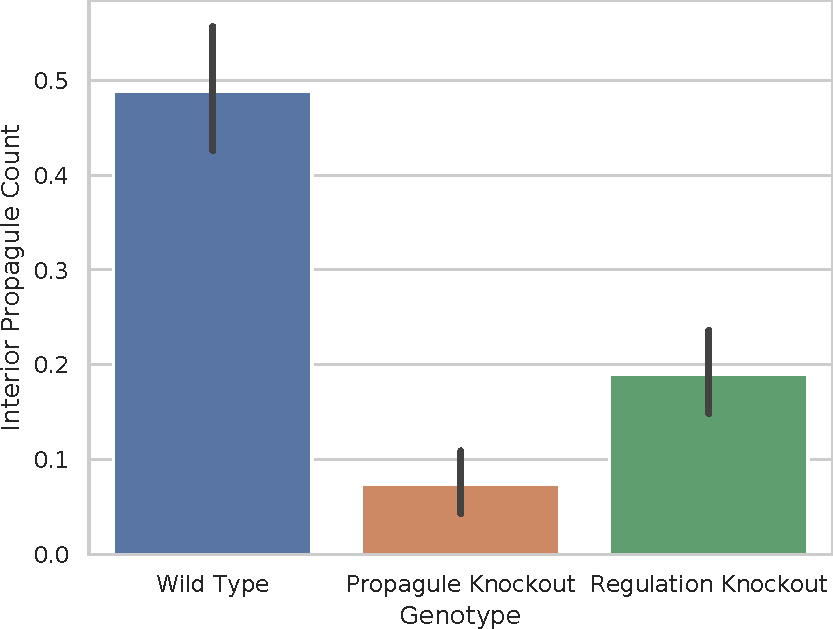
\includegraphics[width=\linewidth]{knockout/interior_propagule/title=interior_propagules+_data_hathash_hash=bb0fa6254f1b7398+_script_fullcat_hash=f738b363bea8c98a+_source_hash=53a2252-clean+ext=}%
\caption{Interior propagule rate by genotype}
\label{fig:interior_propagule_rate}
\end{subfigure}
\end{minipage}%
\hspace*{\fill}


\caption{
Analysis of a wild type strain evolved under the ``Nested-Wave'' treatment exhibiting interior propagule generation, comparing against knockouts of gene regulation and explicitly propagule-generating reproduction instructions.
Figure \ref{fig:wt_timelapse} traces the wild type life history.
Level-one groups are by differentiated by grayscale tone and separated by solid black borders.
Level-zero groups are by separated by dashed gray borders.
In each example, the focal parent level-one group is colored purple and the focal offspring group orange.
Figure \ref{fig:regulation_visualizations} depicts gene regulation at each of a cell's four directional SignalGP instances using a PCA mapping from regulatory state to three-dimensional RGB coordinates, calculated uniquely for each level-one same-channel signaling group.
Black borders divide level-one same-channel signaling groups and white borders divide level-zero same-channel signaling groups.
Endogenous daughter groups annotated with yellow arrows.
Figure \ref{fig:interior_propagule_rate} compares the mean number of interior propagules observed per level-one same-channel signaling group.
Error bars indicate 95\% confidence.
View an animation of wild type gene regulation at \url{https://mmore500.com/hopto/t}.
View the wild type strain in a live in-browser simulation at \url{https://mmore500.com/hopto/g}.
}
\label{fig:ko-interior_propagule}
\end{center}
\end{figure}


What mechanism determines the localization and timing of the propagule placement obseved in life history example \ref{fig:lifecycle-burst}?
This wild type strain exhibits an irregular, but somewhat concentric, spatial pattern of gene regulation illustrated in Figure \ref{fig:interior_propagule-wt}.
In time-series animation, provided in supplementary material, gene regulation appears to fluctuate dynamically.

To assess mechanistic and adaptive role of gene regulation in this strain, we prepared two knockout strains.
In the first, all gene regulation instructions were replaced with \textbf{Nop} instructions (so that gene regulation values would remain default).
In the second, the reproduction instructions to spawn a propagule were replaced with \textbf{Nop} instructions.
Figures \ref{fig:interior_propagule-ko-regulation} and \ref{fig:interior_propagule-ko-propagule} depict the gene regulation phenotypes of these strains.

Figure \ref{fig:interior_propagule_rate} compares interior propagule generation between the strains, confirming the direct mechanistic role of gene regulation in promoting interior propagule generation ($p < 0.05$; bootstrap test).
[TODO just lookin' at non-overlapping 95\% CI's y'all]

In head-to-head match-ups, the wild type strain outcompetes both the regulation-knockout ($20/20$; $p < 0.001$; two-tailed exact test) and the propagule-knockout strains
($20/20$; $p < 0.001$; two-tailed exact test).
The deficiency of the propagule-knockout strain confirms the adaptive role of interior propagule generation.
Likewise, the deficiency of the regulation-knockout strain affirms the adaptive role of gene regulation in the focal wild type strain.

\subsection{Case Study: Gradient-conditioned Cell Behavior} \label{sec:gradient-conditioned-behavior}

\begin{figure}[!htbp]
\begin{center}

\centering

\hspace*{\fill}%
\begin{minipage}[t]{0.05\columnwidth}
\vspace{0pt} % for alignment
\rotatebox{90}{Resource Stockpile}%
\end{minipage}%
\hfill
\begin{minipage}[t]{0.45\columnwidth}
\centering
\vspace{0pt} % for alignment
\adjincludegraphics[width=\textwidth, trim={{.0\width} {.0\width} {.5\width} {.5\width}}, clip]{knockout/stockpiletrigger-sharing/wildtype/seed=1+title=stockpile_viz+treat=resource-wave__channelsense-yes__nlev-two+update=7172+_data_hathash_hash=d856da4ae5863122+_script_fullcat_hash=4c8152cbf92e0da6+_source_hash=53a2252-clean+ext=}%
\end{minipage}%
\hfill
\begin{minipage}[t]{0.45\columnwidth}
\centering
\vspace{0pt} % for alignment
\adjincludegraphics[width=\textwidth, trim={{.0\width} {.0\width} {.5\width} {.5\width}}, clip]{knockout/stockpiletrigger-sharing/knockout/seed=1+title=stockpile_viz+treat=resource-wave__channelsense-yes__nlev-two+update=7172+_data_hathash_hash=6ab6ade50c5344bc+_script_fullcat_hash=4c8152cbf92e0da6+_source_hash=53a2252-clean+ext=}%
\end{minipage}%
\hspace*{\fill}


\hspace*{\fill}%
\begin{minipage}[t]{0.05\columnwidth}
\vspace{0pt} % for alignment
\rotatebox{90}{Resource Sharing}%
\end{minipage}%
\hfill
\begin{minipage}[t]{0.45\columnwidth}
\centering
\vspace{0pt} % for alignment
\adjincludegraphics[width=\textwidth, trim={{.0\width} {.0\width} {.5\width} {.5\width}}, clip]{knockout/stockpiletrigger-sharing/wildtype/seed=1+title=directional_sharing_viz+treat=resource-wave__channelsense-yes__nlev-two+update=7172+_data_hathash_hash=d856da4ae5863122+_script_fullcat_hash=3a1e851383e0ffd4+_source_hash=53a2252-clean+ext=}%
\end{minipage}%
\hfill
\begin{minipage}[t]{0.45\columnwidth}
\centering
\vspace{0pt} % for alignment
\adjincludegraphics[width=\textwidth, trim={{.0\width} {.0\width} {.5\width} {.5\width}}, clip]{knockout/stockpiletrigger-sharing/knockout/seed=1+title=directional_sharing_viz+treat=resource-wave__channelsense-yes__nlev-two+update=7172+_data_hathash_hash=6ab6ade50c5344bc+_script_fullcat_hash=3a1e851383e0ffd4+_source_hash=53a2252-clean+ext=}%
\end{minipage}%
\hspace*{\fill}

\vspace{1.0ex}

\hspace*{\fill}%
\begin{minipage}[t]{0.05\columnwidth}
\vspace{0pt} % for alignment
\end{minipage}%
\hfill
\begin{minipage}[t]{0.45\columnwidth}
\centering
\vspace{0pt} % for alignment
Wild Type
\end{minipage}%
\hfill
\begin{minipage}[t]{0.45\columnwidth}
\centering
\vspace{0pt} % for alignment
Messaging Knockout
\end{minipage}%
\hspace*{\fill}

\vspace{1.0ex}

\caption{
Visualization of phenotypic traits of a wild type strain evolved under the ``Nested-Wave''' treatment and corresponding resource-sensing knockout strain.
In the resource-sharing visualization, color coding represents the amount of incoming shared resource.
White represents no incoming messages and the magenta to blue gradient runs from one incoming message to the maximum observed incoming message traffic.
In the resource stockpile visualization, white represents zero-resource stockpiles, blue represents stockpiles with just under enough resource to reproduce, green represents stockpiles with enough resource to reproduce, and yellow represents more than enough resource to reproduce.
Black borders divide level-one same-channel signaling groups and white borders divide level-zero same-channel signaling groups.
}
\label{fig:ko-stockpiletrigger-sharing}
\end{center}
\end{figure}


We discovered a strain using resource concentration to regulate directionality of resource sharing in a manner somewhat akin to morphogenic patterning.
This strain's wild type outcompeted a variant with knock out of capacity to asses relative richness of neighboring resource stockpiles ($20/20$; $p < 0.001$; two-tailed exact test).
Figure \ref{fig:ko-stockpiletrigger-sharing} contrasts the wild type resource-sharing phenotype  with the more sparse knockout resource-sharing phenotype.

\subsection{Case Study: Morphology} \label{sec:morphology}

\begin{figure}[!htbp]
\begin{center}

\hspace*{\fill}%
\begin{minipage}[t]{0.45\columnwidth}
\centering
\vspace{0pt} % for alignment
\begin{subfigure}[b]{\textwidth}
\adjincludegraphics[width=\textwidth, trim={{.0\width} {.0\width} {.5\width} {.5\width}}, clip]{knockout/morphology/wildtype/seed=1+title=channel_viz+treat=resource-even__channelsense-yes__nlev-two+update=8188+_data_hathash_hash=cb64cdf045bc6049+_script_fullcat_hash=7e789c981e3d0e4f+_source_hash=53a2252-clean+ext=}
\caption{Wild type}
\label{fig:morphology-wt}
\end{subfigure}
\end{minipage}%
\hfill
\begin{minipage}[t]{0.45\columnwidth}
\centering
\vspace{0pt} % for alignment
\begin{subfigure}[b]{\textwidth}
\adjincludegraphics[width=\textwidth, trim={{.0\width} {.0\width} {.5\width} {.5\width}}, clip]{knockout/morphology/knockout/seed=1+title=channel_viz+treat=resource-even__channelsense-yes__nlev-two+update=8188+_data_hathash_hash=9a4119947348e91d+_script_fullcat_hash=7e789c981e3d0e4f+_source_hash=53a2252-clean+ext=}%
\caption{Messaging knockout}
\label{fig:morphology-ko}
\end{subfigure}
\end{minipage}%
\hspace*{\fill}

\hspace*{\fill}%
\begin{minipage}[t]{\columnwidth}
\centering
\vspace{0pt} % for alignment
\begin{subfigure}[b]{\textwidth}
\adjincludegraphics[width=\textwidth]{knockout/morphology/title=group_shape+_data_hathash_hash=cb1733796dea778f+_script_fullcat_hash=68cf35a1759c64ac+_source_hash=53a2252-clean+ext=}
\caption{Distribution of level-zero same-channel neighbor counts}
\label{fig:morphology-shape}
\end{subfigure}
\end{minipage}%
\hspace*{\fill}

\caption{
Comparison of a wild type strain with stringy level-zero same-channel signaling networks and the corresponding intracellular-messaging knockout strain.
Subfigures \ref{fig:morphology-wt} and \ref{fig:morphology-ko} visualize same-channel signaling network layouts;
color hue denotes and black borders divide level-one same-channel signaling networks while
color saturation denotes and white borders divide level-zero same-channel signaling networks.
Subfigure \ref{fig:morphology-shape} quantifies the morphological effect of the
intracellular-messaging knockout.
Error bars indicate 95\% confidence.
}
\label{fig:ko-morphology}
\end{center}
\end{figure}


One of the more striking examples of genetically-encoded same-channel signaling network patterning, in which level-zero same-channel signaling groups arranged as elongated strings, arose in a even treatment replicate.
Figure \ref{fig:morphology-wt} provides a snapshot of this strain's same-channel signaling morphology.
Knocking out intracell messaging disrupts the stringy arrangement of same-channel signaling groups, shown in Figure \ref{fig:morphology-ko}.
Figure \ref{fig:morphology-shape} confirms the genetic basis of the trait.
Cells from the wild-type strain more often neighbor only zero or one level-zero same-channel cells ($p < 0.05$; bootstrap test).
[TODO just lookin' at non-overlapping 95\% CI's y'all]
In contrast, knockout strain cells more frequently neighbor three or four level-zero same-channel cells ($p < 0.05$; bootstrap test).
[TODO just lookin' at non-overlapping 95\% CI's y'all]

However, competition experiments between the wild type and knockout strain failed to establish a fitness differential ($6/20$).
Thus, it seems this trait emerged either by drift, as the genetic background of a selective sweep, or --- perhaps less likely --- was advantageous against a divergent competitor earlier in evolutionary history.

\subsection{Case Studies: Cell-cell Messaging} \label{sec:cell-cell-messaging}

\begin{figure*}[!htbp]
\begin{center}

\begin{minipage}[t]{\columnwidth}
\hspace*{\fill}%
\begin{minipage}[t]{0.05\columnwidth}
\vspace{0pt} % for alignment
\rotatebox{90}{Messaging}%
\end{minipage}%
\hfill
\begin{minipage}[t]{0.45\columnwidth}
\centering
\vspace{0pt} % for alignment
\adjincludegraphics[width=\textwidth, trim={{.0\width} {.0\width} {.5\width} {.5\width}}, clip]{knockout/intermessaging-sharing/wildtype/seed=1+title=directional_messaging_viz+treat=resource-wave__channelsense-yes__nlev-onebig+update=7172+_data_hathash_hash=f9e2a8ff33bf7745+_script_fullcat_hash=6b7e0389992dd616+_source_hash=53a2252-clean+ext=}%
\end{minipage}%
\hfill
\begin{minipage}[t]{0.45\columnwidth}
\centering
\vspace{0pt} % for alignment
\adjincludegraphics[width=\textwidth, trim={{.0\width} {.0\width} {.5\width} {.5\width}}, clip]{knockout/intermessaging-sharing/knockout/seed=1+title=directional_messaging_viz+treat=resource-wave__channelsense-yes__nlev-onebig+update=7172+_data_hathash_hash=ffdeb1c77dd012e1+_script_fullcat_hash=6b7e0389992dd616+_source_hash=53a2252-clean+ext=}%
\end{minipage}%
\hspace*{\fill}

\hspace*{\fill}%
\begin{minipage}[t]{0.05\columnwidth}
\vspace{0pt} % for alignment
\rotatebox{90}{Resource Sharing}%
\end{minipage}%
\hfill
\begin{minipage}[t]{0.45\columnwidth}
\centering
\vspace{0pt} % for alignment
\adjincludegraphics[width=\textwidth, trim={{.0\width} {.0\width} {.5\width} {.5\width}}, clip]{knockout/intermessaging-sharing/wildtype/seed=1+title=directional_sharing_viz+treat=resource-wave__channelsense-yes__nlev-onebig+update=7172+_data_hathash_hash=f9e2a8ff33bf7745+_script_fullcat_hash=3a1e851383e0ffd4+_source_hash=53a2252-clean+ext=}%
\end{minipage}%
\hfill
\begin{minipage}[t]{0.45\columnwidth}
\centering
\vspace{0pt} % for alignment
\adjincludegraphics[width=\textwidth, trim={{.0\width} {.0\width} {.5\width} {.5\width}}, clip]{knockout/intermessaging-sharing/knockout/seed=1+title=directional_sharing_viz+treat=resource-wave__channelsense-yes__nlev-onebig+update=7172+_data_hathash_hash=ffdeb1c77dd012e1+_script_fullcat_hash=3a1e851383e0ffd4+_source_hash=53a2252-clean+ext=}%
\end{minipage}%
\hspace*{\fill}

\hspace*{\fill}%
\begin{minipage}[t]{0.05\columnwidth}
\vspace{0pt} % for alignment
\rotatebox{90}{Resource Stockpile}%
\end{minipage}%
\hfill
\begin{minipage}[t]{0.45\columnwidth}
\centering
\vspace{0pt} % for alignment
\adjincludegraphics[width=\textwidth, trim={{.0\width} {.0\width} {.5\width} {.5\width}}, clip]{knockout/intermessaging-sharing/wildtype/seed=1+title=stockpile_viz+treat=resource-wave__channelsense-yes__nlev-onebig+update=7172+_data_hathash_hash=f9e2a8ff33bf7745+_script_fullcat_hash=4c8152cbf92e0da6+_source_hash=53a2252-clean+ext=}%
\end{minipage}%
\hfill
\begin{minipage}[t]{0.45\columnwidth}
\centering
\vspace{0pt} % for alignment
\adjincludegraphics[width=\textwidth, trim={{.0\width} {.0\width} {.5\width} {.5\width}}, clip]{knockout/intermessaging-sharing/knockout/seed=1+title=stockpile_viz+treat=resource-wave__channelsense-yes__nlev-onebig+update=7172+_data_hathash_hash=ffdeb1c77dd012e1+_script_fullcat_hash=4c8152cbf92e0da6+_source_hash=53a2252-clean+ext=}%
\end{minipage}%
\hspace*{\fill}

\vspace{1.0ex}

\hspace*{\fill}%
\begin{minipage}[t]{0.05\columnwidth}
\vspace{0pt} % for alignment
\end{minipage}%
\hfill
\begin{minipage}[t]{0.45\columnwidth}
\centering
\vspace{0pt} % for alignment
Wild Type
\end{minipage}%
\hfill
\begin{minipage}[t]{0.45\columnwidth}
\centering
\vspace{0pt} % for alignment
Messaging Knockout
\end{minipage}%
\hspace*{\fill}

\vspace{1.0ex}

\begin{subfigure}{\columnwidth}
  \caption{Phenotype visualizations}
\end{subfigure}

\end{minipage}%
\begin{minipage}[t]{\columnwidth}

\hspace*{\fill}%
\begin{minipage}[t]{\textwidth}
\centering
\vspace{0pt} % for alignment
\begin{subfigure}[b]{\textwidth}
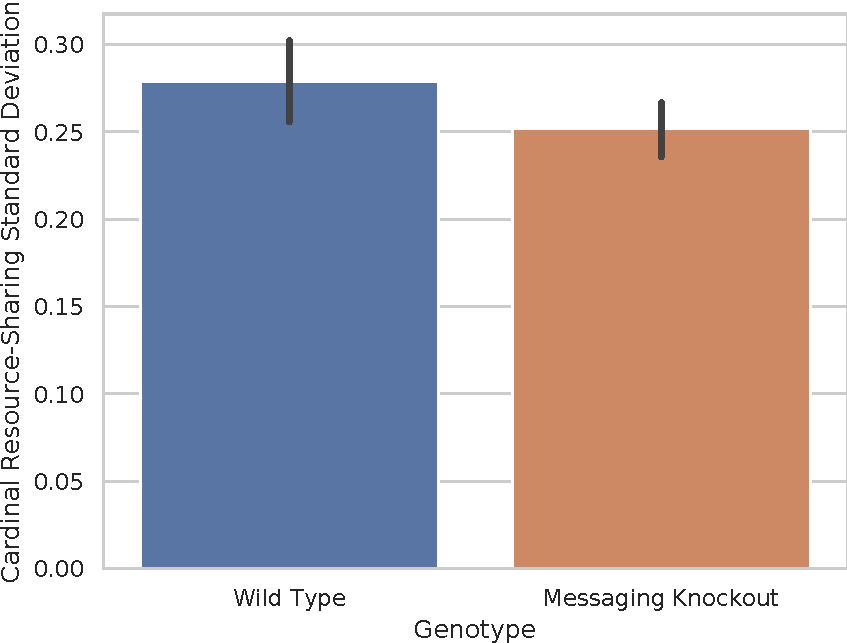
\includegraphics[width=\textwidth]{knockout/intermessaging-sharing/title=sharingdirection+_data_hathash_hash=59f6520a17fb3ad8+_script_fullcat_hash=97aad8dce5e50084+_source_hash=53a2252-clean+ext=}%
\caption{Net sharing direction variance}
\label{fig:TODO}
\end{subfigure}
\end{minipage}%
\hfill
\begin{minipage}[t]{\textwidth}
\centering
\vspace{0pt} % for alignment
\begin{subfigure}[b]{\textwidth}
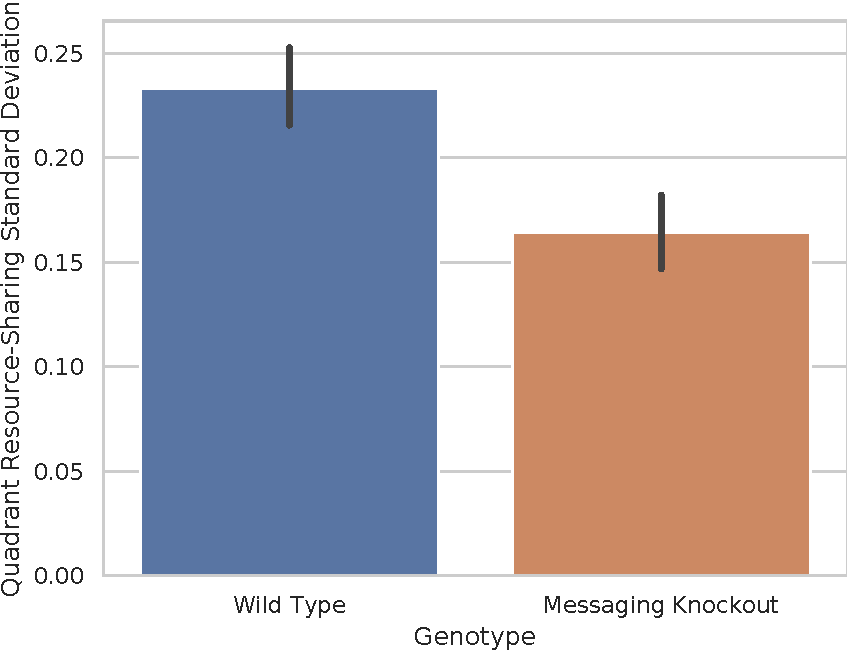
\includegraphics[width=\textwidth]{knockout/intermessaging-sharing/title=sharingquadrant+_data_hathash_hash=586f3c805332c323+_script_fullcat_hash=6e8aa37a96d9d7a9+_source_hash=53a2252-clean+ext=}%
\caption{Net sharing localization variance}
\label{fig:TODO}
\end{subfigure}
\end{minipage}%
\hfill
\begin{minipage}[t]{\textwidth}
\centering
\vspace{0pt} % for alignment
\begin{subfigure}[b]{\textwidth}
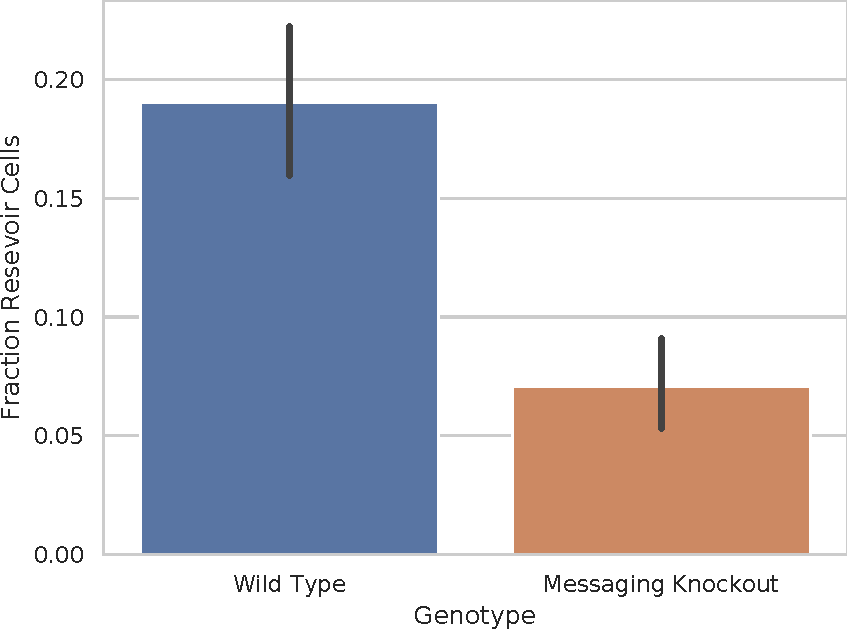
\includegraphics[width=\textwidth]{knockout/intermessaging-sharing/title=fractionresevoir+_data_hathash_hash=7ce9af7e8fe0699b+_script_fullcat_hash=da31ee3af7ae0208+_source_hash=53a2252-clean+ext=}%
\caption{Fraction of cells with enough resource to reproduce}
\label{fig:TODO}
\end{subfigure}
\end{minipage}%
\hspace*{\fill}
\end{minipage}

\caption{
TODO
}
\label{fig:ko-apoptosis}
\end{center}
\end{figure*}


We analyzed the phenotypic and fitness implications of cell-cell messaging in two strains: strain A, evolved under the flat treatment, and strain B, evolved under the nested treatment.

Figure \ref{fig:ko-intermessaging-sharing-phen} depicts the cell-cell messaging, resource sharing, and resource stockpile phenotypes of wild type strain A side-by-side with corresponding phenotypes of a cell-cell messaging knockout strain.
In the wild type strain, cell-cell messaging emanates from irregular collection of cells --- in some regions, grid-like and in others more sparse --- broadcasting to all neighboring cells.
Resource sharing appears more widespread in the knockout strain than in the wild type.
However, messaging's effects suppressing resource sharing is neither spatially nor directionally homogeneous.
Relative to the knockout strain, cell-cell messaging increases variance in cardinal directionality of net resource sharing (Figure \ref{fig:ko-intermessaging-sharing-direction}; $p < 0.05$; bootstrap test).
Cell-cell messaging also increases variance of resource sharing density with respect to spatial quadrants demarcated by same-channel signaling group's spatial centroid (Figure \ref{fig:ko-intermessaging-sharing-direction}; $p < 0.001$; bootstrap test).
We used competition experiments to confirm the fitness advantage both of cell-cell messaging ($20/20$; $p < 0.001$; two-tailed exact test) and (using a separate knockout strain) resource sharing ($20/20$; $p < 0.001$; two-tailed exact test).
The fitness advantage of irregularized sharing might stem from a corresponding increase in the fraction of cells with enough resource to reproduce stockpiled ($p < 0.05$; bootstrap test).
[TODO just lookin' at non-overlapping 95\% CI's y'all]


\begin{figure*}[!htbp]
\begin{center}


\begin{minipage}[t]{\columnwidth}
\centering
\hspace*{\fill}%
\begin{minipage}[t]{0.05\columnwidth}
\vspace{0pt} % for alignment
\rotatebox{90}{Messaging}%
\end{minipage}%
\hfill
\begin{minipage}[t]{0.45\columnwidth}
\centering
\vspace{0pt} % for alignment
\adjincludegraphics[width=\textwidth, trim={{.66\width} {.66\width} {.0\width} {.0\width}}, clip]{knockout/intermessaging-intergroup_border/wildtype/seed=1+title=directional_messaging_viz+treat=resource-wave__channelsense-yes__nlev-two+update=7168+_data_hathash_hash=3895dfa0dd602b4c+_script_fullcat_hash=6b7e0389992dd616+_source_hash=53a2252-clean+ext=}%
\end{minipage}%
\hfill
\begin{minipage}[t]{0.45\columnwidth}
\centering
\vspace{0pt} % for alignment
\adjincludegraphics[width=\textwidth, trim={{.66\width} {.66\width} {.0\width} {.0\width}}, clip]{knockout/intermessaging-intergroup_border/knockout/seed=1+title=directional_messaging_viz+treat=resource-wave__channelsense-yes__nlev-two+update=7168+_data_hathash_hash=24546cc614406803+_script_fullcat_hash=6b7e0389992dd616+_source_hash=53a2252-clean+ext=}%
\end{minipage}%
\hspace*{\fill}

\hspace*{\fill}%
\begin{minipage}[t]{0.05\columnwidth}
\vspace{0pt} % for alignment
\rotatebox{90}{Parent-Propagule}%
\end{minipage}%
\hfill
\begin{minipage}[t]{0.45\columnwidth}
\centering
\vspace{0pt} % for alignment
\adjincludegraphics[width=\textwidth, trim={{.66\width} {.66\width} {.0\width} {.0\width}}, clip]{knockout/intermessaging-intergroup_border/wildtype/seed=1+title=directional_propagule_viz+treat=resource-wave__channelsense-yes__nlev-two+update=7168+_data_hathash_hash=3895dfa0dd602b4c+_script_fullcat_hash=8b1f57a580a67198+_source_hash=53a2252-clean+ext=}%
\end{minipage}%
\hfill
\begin{minipage}[t]{0.45\columnwidth}
\centering
\vspace{0pt} % for alignment
\adjincludegraphics[width=\textwidth, trim={{.66\width} {.66\width} {.0\width} {.0\width}}, clip]{knockout/intermessaging-intergroup_border/knockout/seed=1+title=directional_propagule_viz+treat=resource-wave__channelsense-yes__nlev-two+update=7168+_data_hathash_hash=24546cc614406803+_script_fullcat_hash=8b1f57a580a67198+_source_hash=53a2252-clean+ext=}%
\end{minipage}%
\hspace*{\fill}

\hspace*{\fill}%
\begin{minipage}[t]{0.05\columnwidth}
\vspace{0pt} % for alignment
\rotatebox{90}{Resource Sharing}%
\end{minipage}%
\hfill
\begin{minipage}[t]{0.45\columnwidth}
\centering
\vspace{0pt} % for alignment
\adjincludegraphics[width=\textwidth, trim={{.66\width} {.66\width} {.0\width} {.0\width}}, clip]{knockout/intermessaging-intergroup_border/wildtype/seed=1+title=directional_sharing_viz+treat=resource-wave__channelsense-yes__nlev-two+update=7172+_data_hathash_hash=3895dfa0dd602b4c+_script_fullcat_hash=3a1e851383e0ffd4+_source_hash=53a2252-clean+ext=}%
\end{minipage}%
\hfill
\begin{minipage}[t]{0.45\columnwidth}
\centering
\vspace{0pt} % for alignment
\adjincludegraphics[width=\textwidth, trim={{.66\width} {.66\width} {.0\width} {.0\width}}, clip]{knockout/intermessaging-intergroup_border/knockout/seed=1+title=directional_sharing_viz+treat=resource-wave__channelsense-yes__nlev-two+update=7172+_data_hathash_hash=24546cc614406803+_script_fullcat_hash=3a1e851383e0ffd4+_source_hash=53a2252-clean+ext=}%
\end{minipage}%
\hspace*{\fill}

% \hspace*{\fill}%
% \begin{minipage}[t]{0.05\columnwidth}
% \vspace{0pt} % for alignment
% \rotatebox{90}{Resource Stockpile}%
% \end{minipage}%
% \hfill
% \begin{minipage}[t]{0.45\columnwidth}
% \centering
% \vspace{0pt} % for alignment
% \adjincludegraphics[width=\textwidth, trim={{.66\width} {.66\width} {.0\width} {.0\width}}, clip]{knockout/intermessaging-intergroup_border/wildtype/seed=1+title=stockpile_viz+treat=resource-wave__channelsense-yes__nlev-two+update=7168+_data_hathash_hash=3895dfa0dd602b4c+_script_fullcat_hash=4c8152cbf92e0da6+_source_hash=53a2252-clean+ext=}%
% \end{minipage}%
% \hfill
% \begin{minipage}[t]{0.45\columnwidth}
% \centering
% \vspace{0pt} % for alignment
% \adjincludegraphics[width=\textwidth, trim={{.66\width} {.66\width} {.0\width} {.0\width}}, clip]{knockout/intermessaging-intergroup_border/knockout/seed=1+title=stockpile_viz+treat=resource-wave__channelsense-yes__nlev-two+update=7168+_data_hathash_hash=24546cc614406803+_script_fullcat_hash=4c8152cbf92e0da6+_source_hash=53a2252-clean+ext=}%
% \end{minipage}%
% \hspace*{\fill}

\vspace{1.0ex}

\hspace*{\fill}%
\begin{minipage}[t]{0.05\columnwidth}
\vspace{0pt} % for alignment
\end{minipage}%
\hfill
\begin{minipage}[t]{0.45\columnwidth}
\centering
\vspace{0pt} % for alignment
Wild Type
\end{minipage}%
\hfill
\begin{minipage}[t]{0.45\columnwidth}
\centering
\vspace{0pt} % for alignment
Messaging Knockout
\end{minipage}%
\hspace*{\fill}

\vspace{1.0ex}

\begin{subfigure}{\columnwidth}
  \caption{Phenotype visualizations}
  \label{fig:intermessaging-intergroup_border-phen}
\end{subfigure}

\begin{minipage}[t]{0.8\columnwidth}
\centering
\vspace{0pt} % for alignment
\begin{subfigure}[b]{\textwidth}
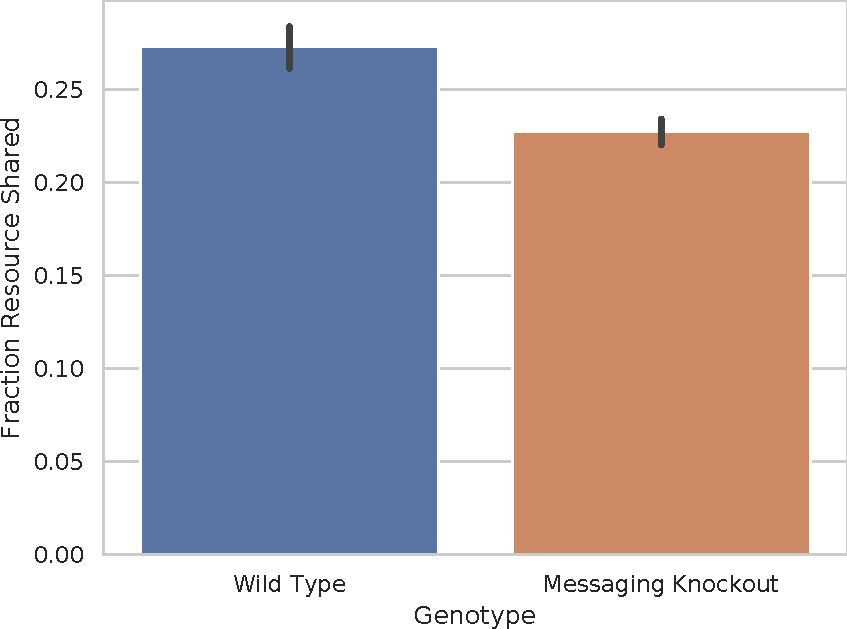
\includegraphics[width=\textwidth]{knockout/intermessaging-intergroup_border/title=sharingfraction+_data_hathash_hash=b0e9f42c3e74cf6a+_script_fullcat_hash=84ce7f4d8802dbab+_source_hash=53a2252-clean+ext=}%
\caption{Resource sharing}
\label{fig:intermessaging-intergroup_border-sharing}
\end{subfigure}
\end{minipage}%

\vspace{1ex}

\hspace*{\fill}%
\begin{minipage}[t]{0.8\columnwidth}
\centering
\vspace{0pt} % for alignment
\begin{subfigure}[b]{\textwidth}
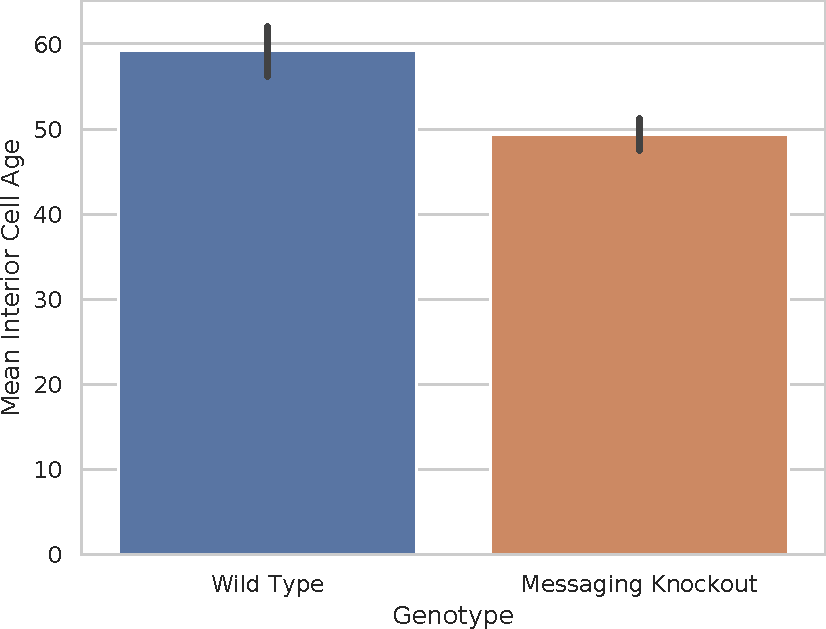
\includegraphics[width=\textwidth]{knockout/intermessaging-intergroup_border/title=cellageraw+_data_hathash_hash=ef9f5e984a40fbf6+_script_fullcat_hash=1faec38cdb6bd1de+_source_hash=53a2252-clean+ext=}%
\caption{Interior cell age}
\label{fig:intermessaging-intergroup_border-cellage}
\end{subfigure}
\end{minipage}%
\hspace*{\fill}

\end{minipage}%
\begin{minipage}[t]{\columnwidth}
\centering

\hspace*{\fill}%
\begin{minipage}[t]{0.8\columnwidth}
\centering
\vspace{0pt} % for alignment
\begin{subfigure}[b]{\textwidth}
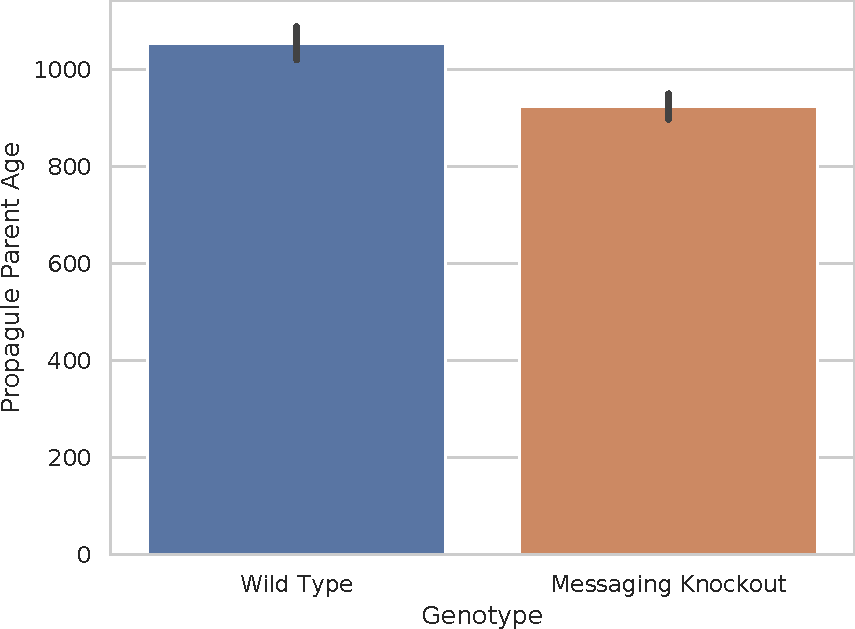
\includegraphics[width=\textwidth]{knockout/intermessaging-intergroup_border/title=parentage+_data_hathash_hash=974d02d36b7dba1a+_script_fullcat_hash=7ee3d274683ffdb2+_source_hash=53a2252-clean+ext=}%
\caption{Propagule parent age}
\label{fig:intermessaging-intergroup_border-pparentage}
\end{subfigure}
\end{minipage}%
\hspace*{\fill}

\vspace{1ex}

\hspace*{\fill}%
\begin{minipage}[t]{0.8\columnwidth}
\centering
\vspace{0pt} % for alignment
\begin{subfigure}[b]{\textwidth}
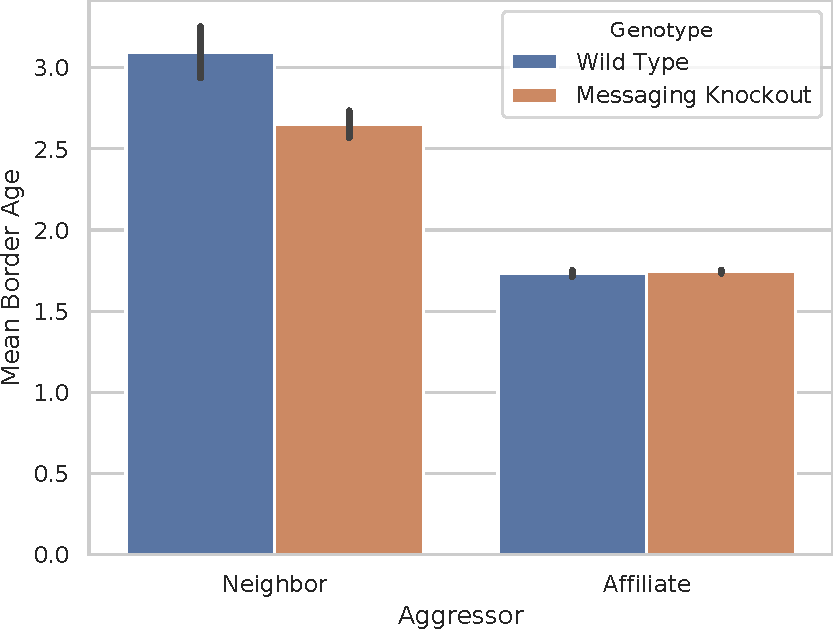
\includegraphics[width=\textwidth]{knockout/intermessaging-intergroup_border/title=comboborderage+_data_hathash_hash=8369fa84222d9217+_script_fullcat_hash=c576822d0876c8a8+_source_hash=53a2252-clean+ext=}%
\caption{Border age}
\label{fig:intermessaging-intergroup_border-borderage}
\end{subfigure}
\end{minipage}%
\hspace*{\fill}

\vspace{1ex}

\hspace*{\fill}%
\begin{minipage}[t]{0.8\columnwidth}
\centering
\vspace{0pt} % for alignment
\begin{subfigure}[b]{\textwidth}
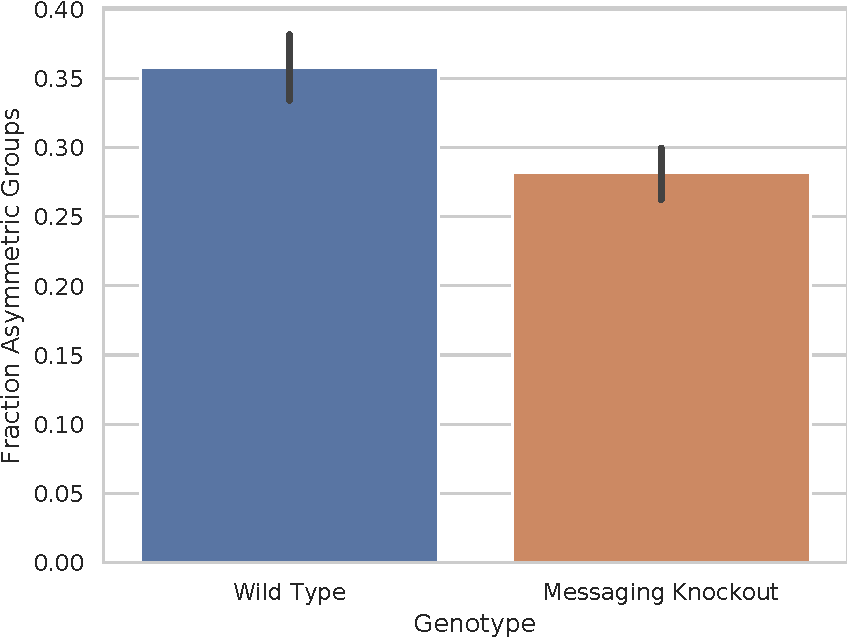
\includegraphics[width=\textwidth]{knockout/intermessaging-intergroup_border/title=metabolismasymmetry+_data_hathash_hash=3ce8f7b8474367f3+_script_fullcat_hash=0329612f3b158905+_source_hash=53a2252-clean+ext=}%
\caption{Asymmetric border metabolism}
\label{fig:intermessaging-intergroup_border-metabolism}
\end{subfigure}
\end{minipage}%
\hspace*{\fill}

\caption{
Comparison of wild type strain and corresponding intercell messaging knockout strain.
Subfigure \ref{fig:intermessaging-intergroup_border-phen} visualizes phenotypic traits in the wild type and knockout strain.
In the messaging visualization, color coding represents the volume of incoming messages.
White represents no incoming messages and the magenta to blue gradient runs from one incoming message to the maximum observed incoming message traffic.
In the resource sharing visualization, this same color coding represents the amount of incoming shared resource.
Solid black borders divide level-one same-channel signaling networks and dotted light gray borders divide level-zero same-channel signaling networks.
Subfigures \ref{fig:intermessaging-intergroup_border-sharing}, \ref{fig:intermessaging-intergroup_border-cellage}, \ref{fig:intermessaging-intergroup_border-pparentage}, \ref{fig:intermessaging-intergroup_border-borderage}, and \ref{fig:intermessaging-intergroup_border-metabolism} quantify knockout effects on various phenotypic traits.
Error bars indicate 95\% confidence.
}
\label{fig:ko-intermessaging-intergroup_border}
\end{minipage}

\end{center}
\end{figure*}


Figure \ref{fig:intermessaging-intergroup_border-phen} compares the cell-cell messaging, resource sharing, and parent-propagule phenotypes between wild type and cell-cell messaging knockout variants of strain B.
Cell-cell messaging volume appears generally uniform in the interiors of same-channel signaling groups, but some group-group borders --- largely, but not entirely parent-propagule interfaces --- manifest somewhat depressed cell-cell messaging overlaid with an alternating motif of elevated cell-cell messaging.
We affirmed the adaptiveness of cell-cell messaging in this strain through competition experiments between wild type and knockout variants ($19/20$; $p < 0.001$; two-tailed exact test).
The gene activated by cell-cell messaging in this strain contains a share resource instruction and, indeed, we observed significantly greater net resource sharing in the wild type strain (Figure \ref{fig:intermessaging-intergroup_border-sharing}; non-overlapping 95\% CI).
However, that same gene also contains a reproduction-inhibiting instruction, leading us to investigate whether cell-cell messaging could influence a broader set of phenotypic traits.

Cell-cell messaging in the wild type strain appears to be associated with a somewhat drawn out collective life history.
The wild-type strain exhibits significantly greater mean cell age (Figure \ref{fig:intermessaging-intergroup_border-sharing}, $n=20$, non-overlapping 95\% CI) and mean propagule parent group age (Figure \ref{fig:intermessaging-intergroup_border-pparentage}; $n=20$; non-overlapping 95\% CI).
This strain exhibits the ``sweep'' life history described in Figure \ref{fig:lifestyle-sweep}, so propagule generation can be largely or entirely destructive to the parent group.
So, the increase in mean cell age could plausibly be attributable to delayed propagule genesis or, alternatively, delayed propagule genesis could arise from other factors retarding life history.

Cell-cell messaging not only enables functional coordination within cellular collectives but could might reify adaptive communication among cellular collectives.
This possibility motivated us to take a closer look at interactions between same-channel signaling network groups.
We anecdotally observed that contiguous bands of low cell turnover frequently arose along parent-propagule borders, but also occasionally between other same-channel signaling network groups.
We measured the mean age of perturbed borders (e.g., updates elapsed between perturbations) along non-parent-child borders.
Figure \ref{fig:intermessaging-intergroup_border-borderage} splits this statistic out between borders that were disrupted by members of the same-channel signaling network flanking the border (``affiliate'') or by a member of a third same-channel signaling network (``neighbor'').
In both wild type and knockout strains, there was significantly more recent turnover in the absence of intrusion by a third same-channel signaling network (non-overlapping 95\% CI).
Although the wild type strain exhibits slightly higher turnover rates on borders plied by only two groups, borders invaded by a third group are significantly more stale than the knockout strain (non-overlapping 95\% CI).
This observation could be consistent with a general slowing of turnover as a same-channel signaling networks age, asymmetrical antagonism towards same-channel signaling group neighbors (perhaps arising from a primitive tit-for-tat policy), or some combination of these explanations.

So, does metabolism fluctuate uniformly across a same-channel signaling network's borders or can metabolism differ significantly across a group's non-parent-child neighbor groups at a single time point?
To assess this question, we used Kruskal-Wallis tests (with Bonferroni correction) to screen for same-channel signaling network groups with border metabolic distributions that differed significantly between neighboring non-propagule-parent same-channel signaling network groups.
For each same-channel signaling network group, we calculated mean per-border-cell birth rate at the interface of each of its non-propagule-parent neighbor groups.
We compared sets of observations taken from each neighbor every eighth update over 256 updates.
Groups with significantly distinguishable border metabolism distributions occurred in both the wild type and messaging knockout strains.
However, a significantly higher proportion of groups exhibited asymmetric border metabolism with non-parent-child groups (Figure \ref{fig:intermessaging-intergroup_border-metabolism}; $p < 0.001$; $n=20$; bootstrap test).
In this case, messaging between cells registered to different propagule-parent same-channel signaling network groups seems unlikely to directly underlie this phenomenon because execution of the gene targeted by messages triggers resource-sharing to the sender, which we seldom observed.
However, cell-cell messaging within a same-channel signaling network does appear to bolster asymmetrical group-group antagonism, perhaps by conducting tit-for-tat behavior or by altering population demography.

\subsection{Case Studies: Apoptosis} \label{sec:apoptosis}

\begin{figure}[!htbp]
\begin{center}

\hspace*{\fill}%
\begin{minipage}[t]{0.05\columnwidth}
\vspace{0pt} % for alignment
\rotatebox{90}{Strain A}%
\end{minipage}%
\hfill
\begin{minipage}[t]{0.45\columnwidth}
\centering
\vspace{0pt} % for alignment
\adjincludegraphics[width=\textwidth, trim={{.5\width} {.5\width} {.0\width} {.0\width}}, clip]{knockout/apoptosis/wildtype/seed=1+title=channel_viz+treat=resource-even__channelsense-yes__nlev-two+update=262144+_data_hathash_hash=9b92a609c3309033+_script_fullcat_hash=7e789c981e3d0e4f+_source_hash=53a2252-clean+ext=}%
\end{minipage}%
\hfill
\begin{minipage}[t]{0.45\columnwidth}
\centering
\vspace{0pt} % for alignment
\adjincludegraphics[width=\textwidth, trim={{.5\width} {.5\width} {.0\width} {.0\width}}, clip]{knockout/apoptosis/knockout/seed=1+title=channel_viz+treat=resource-even__channelsense-yes__nlev-two+update=262144+_data_hathash_hash=900abeef45bb9133+_script_fullcat_hash=7e789c981e3d0e4f+_source_hash=53a2252-clean+ext=}%
\end{minipage}%
\hspace*{\fill}

\hspace*{\fill}%
\begin{minipage}[t]{0.05\columnwidth}
\vspace{0pt} % for alignment
\rotatebox{90}{Strain B}%
\hfill
\end{minipage}%
\hfill
\begin{minipage}[t]{0.45\columnwidth}
\centering
\vspace{0pt} % for alignment
\adjincludegraphics[width=\textwidth, trim={{.5\width} {.5\width} {.0\width} {.0\width}}, clip]{knockout/apoptosis/wildtype/seed=1+title=channel_viz+treat=resource-wave__channelsense-yes__nlev-onebig+update=8188+_data_hathash_hash=3465df2fce2dc5f4+_script_fullcat_hash=7e789c981e3d0e4f+_source_hash=53a2252-clean+ext=}
\end{minipage}%
\hfill
\begin{minipage}[t]{0.45\columnwidth}
\centering
\vspace{0pt} % for alignment
\adjincludegraphics[width=\textwidth, trim={{.5\width} {.5\width} {.0\width} {.0\width}}, clip]{knockout/apoptosis/knockout/seed=1+title=channel_viz+treat=resource-wave__channelsense-yes__nlev-onebig+update=8188+_data_hathash_hash=9c40470beee1c5b5+_script_fullcat_hash=7e789c981e3d0e4f+_source_hash=53a2252-clean+ext=}%
\end{minipage}%
\hspace*{\fill}

\vspace{1.0ex}

\hspace*{\fill}%
\begin{minipage}[t]{0.05\columnwidth}
\vspace{0pt} % for alignment
\end{minipage}%
\hfill
\begin{minipage}[t]{0.45\columnwidth}
\centering
\vspace{0pt} % for alignment
Wild Type
\end{minipage}%
\hfill
\begin{minipage}[t]{0.45\columnwidth}
\centering
\vspace{0pt} % for alignment
Apoptosis Knockout
\end{minipage}%
\hspace*{\fill}

\caption{
Comparison of wild type strains and corresponding apoptosis knockout strains.
In all visualizations, color hue denotes and black borders divide highest-level same-channel signaling networks.
In Replicate A visualizations, color saturation denotes and white borders divide level-zero same-channel signaling networks.
(Replicate B evolved under the flat treatment).
Black tiles are dead.
}
\label{fig:ko-apoptosis}
\end{center}
\end{figure}


Screening replicate evolutionary runs by apoptosis rate flagged two strains with several orders of magnitude greater activity.
In strain A, evolved under the even treatment, apoptosis accounts for 2\% of cell mortality.
In strain B, evolved under the flat treatment, 15\% of mortality is due to apoptosis.

To test the adaptive role of apoptosis in these strains, we performed competition experiments against apoptosis knockout strains, in which all apoptosis instructions were substituted for Nop instructions.
Figure \ref{fig:ko-apoptosis} compares the same-channel wild type phenotypes of these strains to their corresponding knockouts.

Apoptosis contributed significantly to fitness in both strains (strain A: $18/20$, $p < 0.001$, two-tailed exact test; strain B: $20/20$, $p < 0.001$, two-tailed exact test).
The success of strategies incorporating cell suicide is characteristic of evolutionary conditions favoring altruism, such kin selection or a transition from cell-level to collective individuality.
